\label{validation}

In order to ensure that the tuning results were valid across laser travel speeds and power levels a range of 8 other parameters were compared, the values used can be seen in Table \ref{tab:val_parameters}.
\begin{table}[!htb]
	\centering
	\caption{Validation processing parameters}
	\label{tab:val_parameters}
		\begin{tabular}{|c|c|c|} \hline 
			Exp. Id. & Scan speed (mm/min) & Laser Power (W) \\ \hline
			1 & 762 & 1000 \\ \hline  % 0
			2 & 762 & 1500 \\ \hline  % 1
			3 & 762 & 1250 \\ \hline  % 2
			4 & 1143 & 1250 \\ \hline % 3
			5 & 1143 & 1500 \\ \hline  % 5
			6 & 1524 & 1750 \\ \hline  % 6
			7 & 1524 & 1500 \\ \hline  % 7
			8 & 1524 & 2000 \\ \hline  % 8
		\end{tabular}
\end{table}

% \begin{figure}[!htb]\centering
% 	\begin{subfigure}[c]{0.45\textwidth}\centering
% 	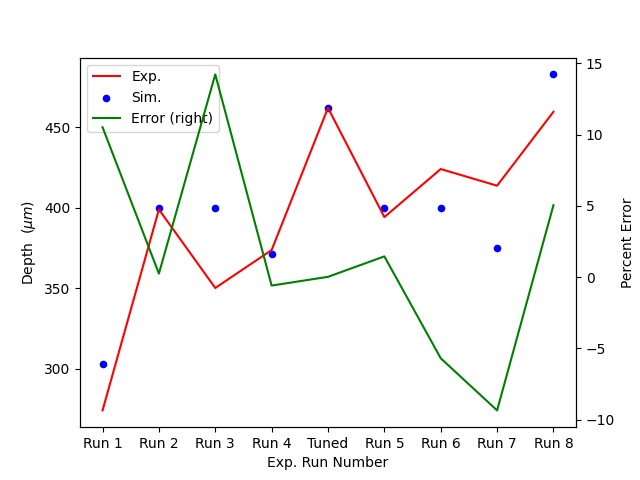
\includegraphics[width=\textwidth]{melt_track_val_depth}
% 	\caption{Melt track depth}
% 	\label{fig:melt_track_val_depth}
% 	\end{subfigure}\hfill{}
% 		\begin{subfigure}[c]{0.45\textwidth}\centering
% 		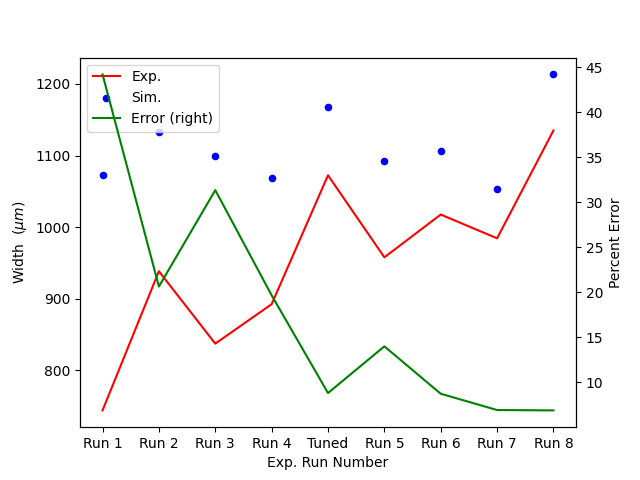
\includegraphics[width=\textwidth]{melt_track_val_width}
% 		\caption{Melt track width}
% 		\label{fig:melt_track_val_width}
% 		\end{subfigure}
% 	\caption{Comparison of experimental and simulated results for validation points}
% 	\label{fig:melt_track_val}
% \end{figure}